\subsubsection{Product Browser}
The Product Browser is found in the second tab in our HomeActivity. It was
implemented in the following manner:
\begin{description}
\item[Product Search] This was implemented in two seperate Fragments,
LocationSearchFragment and ProductSearchFragment. LocationSearchFragment allows
the user to specify the locations at which products must be searched for and is
the first Fragment to be displayed in the tab. Clicking on the search button in
it takes the user to the ProductSearchFragment which allows the user to specify
the products or categories to be searched for. Clicking on the search button
here initiates the actual search and takes the user to the BrowseFragment.
\item[Product Viewer] This was implemented as BrowseFragment which displays a
list of the found products. Each list item gives the product's name and price
and is clickable, with a click bringing up an Info Popup. There is also a graph
button present which takes the user to ChartActivity (described in Graph
Viewer).
\item[Info Popup] This was implemented an AlertDialog which displays
information about each product, including:
\begin{itemize}
  \item name,
  \item brand,
  \item size,
  \item price,
  \item date of last scan, and
  \item store scanned at.
\end{itemize} 
The dialog also allows the user to share the product using other applications or
to view the store the product was found at in MapsActivity (described in
Directions Viewer).
\end{description}
\begin{figure}[h!]
\centering
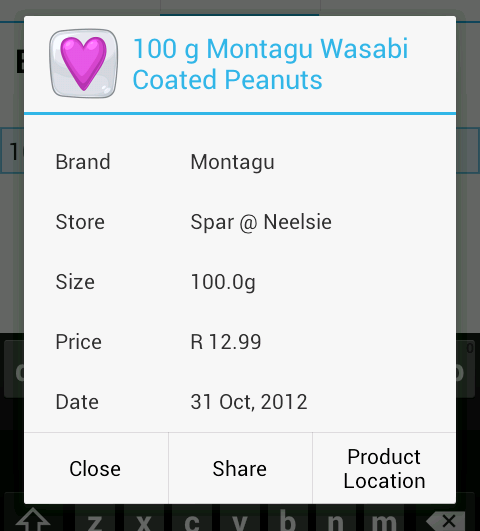
\includegraphics[width=0.3\textwidth]{product-info.png}
\caption{Product info display after a successful search.}
\end{figure}